Молекулярный спектр поглощения паров йода можно наблюдать, используя

\begin{enumerate}
  \item источник сплошного спектра -- лампу накаливания;
  \item поглощаемую среду -- кювету с исследуемым веществом;
  \item спектральный прибор, регистрирующий спектр поглощения -- монохроматор
  УМ-2.
\end{enumerate}

\begin{figure}[h!]
  \centering
  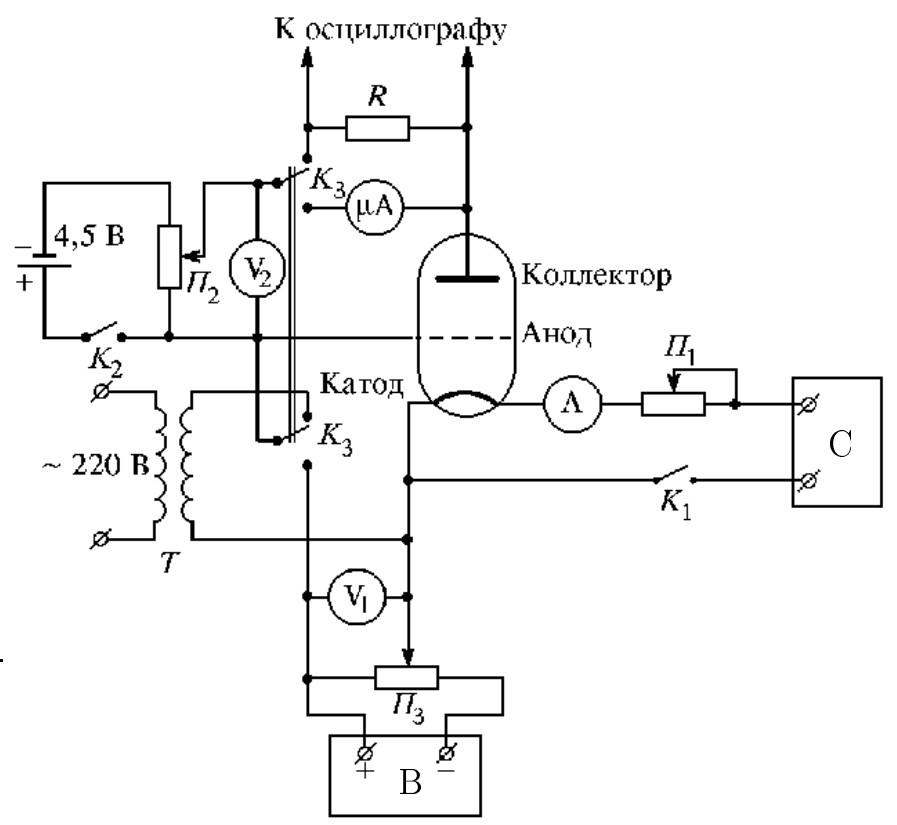
\includegraphics[width=0.9\linewidth]{pic3.png}
  \caption{Градуировка спектрометра}
  \label{pic3}
\end{figure}

В нашей работе спектр поглощения паров йода наблюдается визуально на фоне
сплошного спектра лампы накаливания $1$, питаемой от блока питания 2 (рис.
\ref{pic3}.)

Кювета $3$ с кристаллами йода подогревается нихромовой спиралью, подключенной
вместе с лампой накаливания к блоку питания. Линза $4$ используется как
конденсор.

\begin{figure}[h!]
  \centering
  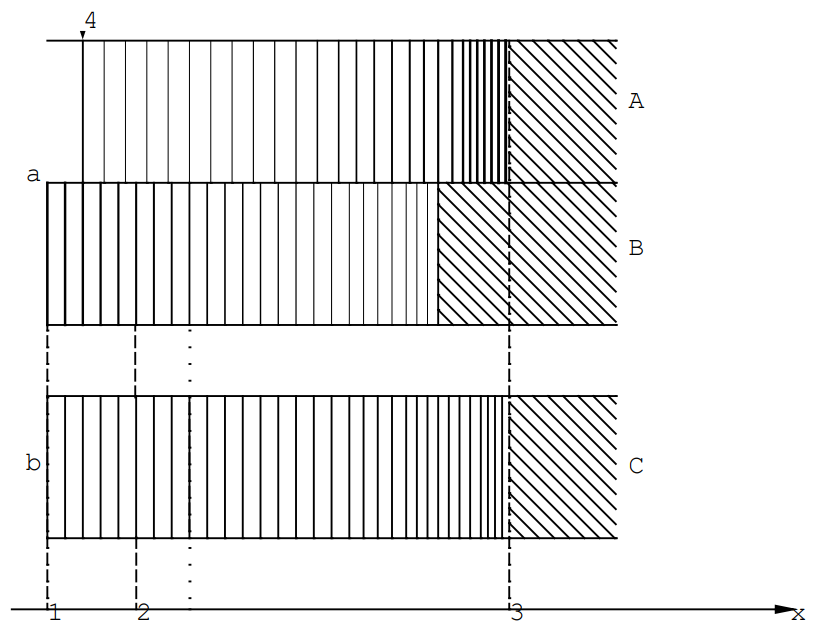
\includegraphics[width=0.9\linewidth]{pic4.png}
  \caption{Градуировка спектрометра}
  \label{pic4}
\end{figure}

В результате подогрева кристаллы йода частично возгоняются, образуя пары с
легкой фиолетовой окраской. Спектрометр позволяет визуально наблюдать линии
поглощения молекул йода на фоне сплошного спектра излучения лампы накаливания
видимой области (рис. \ref{pic4}.)
